\begin{center}
    \vspace*{1.5cm}
    {\fontsize{20}{20}\textbf{Internationella visor}}\\
    \vspace{0.7cm}
    {\fontsize{12}{12}\textit{Om bytisen själv får välja}}
\end{center}
\addtocwithheader{Internationella visor}  % Add entry to TOC and set header\noBackground
\noBackground

\newpage
\resetBackground

\subsubsection*{Skåla med utbytesstudenter}


\begin{tabular}{l l l}
    \textit{Svenska} & - & \hspace{10pt} \textit{Skål} \\
    \textit{Engelska} & - & \hspace{10pt} \textit{Cheers} \\
    \textit{Tyska} & - & \hspace{10pt} \textit{Prost} \\
    \textit{Finska} & - & \hspace{10pt} \textit{Kippis} \\
    \textit{Turkiska} & - & \hspace{10pt} \textit{Şerefe} \\
    \textit{Ungerska} & - & \hspace{10pt} \textit{Egészségedre} \\
    \textit{Japanska} & - & \hspace{10pt} \textit{Kanpai} \\
    \textit{Ryska} & - & \hspace{10pt} \textit{Na zdarovje} \\
    \textit{Kinesiska} & - & \hspace{10pt} \textit{Gan bei} \\
    \textit{Koreanska} & - & \hspace{10pt} \textit{Gun bae} \\
    \textit{Franska} & - & \hspace{10pt} \textit{Santé} \\
    \textit{Skånska} & - & \hspace{10pt} \textit{Skeeool} \\
    \textit{Spanska} & - & \hspace{10pt} \textit{Salud} \\
    \textit{Swahili} & - & \hspace{10pt} \textit{Maisha marefu} \\
    \textit{Filippinska} & - & \hspace{10pt} \textit{Mabuhay} \\
    \textit{Arabiska} & - & \hspace{10pt} \textit{Fisehatak} \\
    \textit{Persiska} & - & \hspace{10pt} \textit{Salam ati} \\
    \textit{Italienska} & - & \hspace{10pt} \textit{Salute} \\
    \textit{Grekiska} & - & \hspace{10pt} \textit{Yiamas} \\
    \textit{Hebreiska} & - & \hspace{10pt} \textit{L’chaim} \\
    \textit{Tjeckiska} & - & \hspace{10pt} \textit{Na zdraví} \\
    \textit{Quenya alviska} & - & \hspace{10pt} \textit{Almien} \\
\end{tabular}


\vissteduatt{Visste du att i Sagan om Ringen talar alverna Sindarin? Därför \\förstår de inte Quenya alviska.}

\newpage

\subsection*{Drunken Sailor} 
\index[alfa]{Drunken Sailor}
\index[anfa]{Drunken Sailor}
% \songinfo{Mel: }

\begin{parse lines}[\noindent]{#1\\}
    What shall we do with the drunken sailor,
    What shall we do with the drunken sailor,
    What shall we do with the drunken sailor,
    Early in the morning?

    Hooray and up she rises,
    Hooray and up she rises,
    Hooray and up she rises,
    Early in the morning!

    Put him in the longboat till he's sober…

    Pull out the plug and wet him all over…

    Put him in the scuppers with a hose-pipe on him…

    Heave him by the leg in a running bowline…

    Shave his belly with a rusty razor…
\end{parse lines}

\newpage

\subsection*{Trink, trink, Brüderlein, trink} 
\index[alfa]{Trink, trink, Brüderlein, trink}
\index[anfa]{Trink, trink, Brüderlein, trink}
% \songinfo{Mel: Bamse\\Sångarstriden 1987}

\begin{parse lines}[\noindent]{#1\\}

    Trink, trink, Brüderlein, trink,
    lass doch die Sorgen zu Haus!
    Trink, trink, Brüderlein, trink,
    bald ist das Leben aus!
    
    ||: Meide den Kummer und meide das Schmerz,
    dann ist das Leben ein Scherz :||
\end{parse lines}

\subsection*{Follow me} 
\index[alfa]{Follow me}
\index[anfa]{This looks like a shot for me}
\songinfo{Mel: Eminem - Without me (refräng)\\
Lundakarnevalen 2022}

\begin{parse lines}[\noindent]{#1\\}
    Now this looks like a shot for me
    So everybody, just follow me
\end{parse lines}


\subsection*{Lisää Vinaa} 
\index[alfa]{Lisää Vinaa}
\index[anfa]{Lisää Vinaa}
\songinfo{Mel: Internationalen}

\begin{parse lines}[\noindent]{#1\\}
    Lisää viinaa mun lasiin,
    lisää laseja pöydälle,
    lisää pöytiä näihin juhliin,
    lisää juhlia kansalle

    Lisää kansaa Suomeen,
    lisää Suomea päälle maan,
    lisää maata Suomelle,
    marssitaan, marssitaan 
    Karjalaan, Karjalaan!
\end{parse lines}

\newpage

\subsection*{Hell and gore} 
\index[alfa]{Hell and gore}
\index[anfa]{Hell and gore}
\songinfo{Mel: Helan går}

\begin{parse lines}[\noindent]{#1\\}
    Hell and Gore
    Chung Hop father Allan, Allan ley
    Hell and Gore
    Chung Hop father Allan ley

    Oh handsome in the hell and tar
    And hell are in the half and four
    Hell and Goooooore………
    Chung Hop father Allan ley

\end{parse lines}


\subsection*{This is the wine} 
\index[alfa]{This is the wine}
\index[anfa]{This is the wine}
\songinfo{Mel: This is the way\\
Lundakarnevalen 2014}

\begin{parse lines}[\noindent]{#1\\}
    This
    This is the wine
    This is the wine we’ll whine about
    When we wake up tomorrow (wakin’ up, wakin’ up)
    This is the wine we’ll whine about!
\end{parse lines}

\vissteduatt{Visste du att E-sektionen vid ett tillfälle hade 28 olika medaljer som\\delades ut?}
\newpage

\subsection*{Minnet} 
\index[alfa]{Minnet}
\index[anfa]{Jag har tappat mitt minne}
\songinfo{Mel: Memory}

\begin{parse lines}[\noindent]{#1\\}
    Minne!
    Jag har tappat mitt minne
    Är jag svensk, eller finne?
    Kommer inte ihåg
    Inne!
    Är jag ut', eller inne?
    Jag har luckor i minne
    - sån där små alkohål
    Men besinn' er,
    man tätar med det brännvin man får,
    fastän minnet och helan går!

    Minne?
    Muisti hävis', mutt' minne?
    juhlista selvisimme
    - muistikatkoja on
    Minne?
    Lähtisin vaikka minne,
    kunhan selvittäisimme
    mitä sattunut on
    Mutta tiedän mä keinon
    mikä auttaapi tuo:
    Ota ryyppy, ja muistis' juo!
\end{parse lines}

%\vissteduatt{visste du att...}

\newpage

\subsection*{A complex world} 
\index[alfa]{A complex world}
\index[anfa]{A complex world}
\songinfo{Mel: A whole new world (from Aladdin) \\
Translated by: León Salueña Martinez BME19}

\begin{parse lines}[\noindent]{#1\\}
    All the pages of proofs
    exasperated they make me,
    laborations convince me:
    My past grades were way too high

    How are you supposed
    to utilise this theorem?
    Appendixes, I've read 'em,
    didn't mention this at all!

    A complex world  
    How the fuck should this be graphed?  
    When all that I underline, and read online,  
    is lost after the exam  
    What will I do?  
    And this is only chapter two...  
    Starting to realise, that I despise,  
    those who told me I need to take this course  

    I can parameterise it... 

    I can help you with C 
    Imaginary exponents  
    Unforgettable moments
    when we study side by side  


    The end's in sight!  
    Just like your mother's was last night
    My studies are organised, prioritised,  
    I stopped procrastinating  
    I've become versed!  
    In solving tortuous PDEs  
    I'm finally safe and sound, a key I found,  
    it laid there in a whole new world: Laplace!

\end{parse lines}

\vissteduatt{Visste du att E-sektionen registrerade på 70-talet en regattabåt så\\att den fick tillstånd att bedriva handel i sjön Sjön? Flera länder\\erkände den, bland annat Norge.}

\newpage

\subsection*{Dansk snapsvisa} 
\index[alfa]{Dansk snapsvisa}
\index[anfa]{Icke nu, men nu!}
\songinfo{Mel: Valfri}

\begin{parse lines}[\noindent]{#1\\}
    Icke nu,
    Icke nu,
    Icke nu,
    men nu!
\end{parse lines}


\subsection*{Finsk snapsvisa} 
\index[alfa]{Finsk snapsvisa}
% \index[anfa]{Icke nu, men nu!}
% \songinfo{Mel: Valfri}

\begin{parse lines}[\noindent]{#1\\}

    ;)
\end{parse lines}


\subsection*{Liang zhi lao hu}
% \index[alfa]{Finsk snapsvisa}
% \index[anfa]{Icke nu, men nu!}
\songinfo{Mel: Broder Jakob}

\begin{parse lines}[\noindent]{#1\\}
    Liang zhi lao hu,
    Liang zhi lao hu
    Pao de kuai,
    Pao de kuai
    Yi zhi mei you yan jing
    Yi zhi mei you er duo
    Zhen qi guai, zhen qi guai    
\end{parse lines}

\vissteduatt{Visste du att 2019 åkte den sista årskullen E:are på utbyte i \\Kina via Kinainriktningen?}

\newpage

\subsection*{Jesus is with us} 
\index[alfa]{Jesus is with us}
\index[anfa]{Jesus is with us}
\songinfo{Mel: Sån't är livet \\
Translated by: León Salueña Martinez BME19}

\begin{parse lines}[\noindent]{#1\\}
    Jesus is with us, he lives in Skövde.  
    He has a Volvo, and fiance  
    He tends his garden, with rhododendron  
    He works a tough job, for decent pay  

    From a young age, he was an odd one  
    When others played war, he would rest  
    But when his best friend, Sven, was wounded  
    Jesus was with him to resurrect  

    Jesus's with us, he lives in Skövde....  

    He went to high school, like all the others  
    He was outstanding, at PE  
    Oh what a great lad, he walked on water
    One time he trekked down, to Miami  

    Jesus's with us, he lives in Skövde....

    During his teen years, he was a loved one
    He got invited, to every feast
    Oh what a great lad, he could turn water
    Into the hard stuff, without yeast

    Jesus's with us, he lives in Skövde.…

\end{parse lines}

\newpage

\subsection*{The Engineers' Drinking Song} 
\index[alfa]{The Engineers' Drinking Song}
\index[anfa]{Den där jäkligt långa låten}
\songinfo{Mel: Battle Hymn of the Republic}

\begin{parse lines}[\noindent]{#1\\}
    Godiva was a lady who through Coventry did ride
    To show the royal villagers her fine and pure white hide
    The most observant man of all, an engineer of course,
    Was the only one who noticed that Godiva rode a horse
    
    We are, we are, we are, we are, we are the Engineers
    We can, we can, we can, we can, demolish forty beers
    Drink rum, drink rum, drink rum all day, and come along with us
    'Cause we don't give a damn for any old man who don't give a damn for us!
    
    She said, I've come a long, long way, and I will go as far
    With the man who takes me from this horse and leads me to a bar
    The men who took her from her steed and led her to a beer
    Were a bleary-eyed surveyor and a drunken engineer
    
    Caesar set out for Egypt at the age of fifty-three
    But Cleopatra's blood was warm, her heart was young and free
    And every night when Julius said good-night at three o'clock
    A Roman Engineer was waiting just around the block!
\end{parse lines}
\newpage
\begin{parse lines}[\noindent]{#1\\}
    The Army and the Navy went out to have some fun
    They went down to the taverns where the fiery liquors run
    But all they found were empties for the Engineers had come
    And traded all their instruments for gallon kegs of rum

    An artsman and an Engineer once found a gallon can
    Said the artsman: “Match me drink for drink, let's see if you're a man”
    They drank three drinks, the artsman fell, his face was turning green
    But the Engineer drank on and said, "It's only gasoline!"

    An Engineer once came to class drunk and very late
    He was carrying a load that you'd expect to ship by freight
    In fact, the only things there were that kept him on his course
    Were the boundary conditions and the Coriolis force

    A physics man from M.I.T. went out and drank his fill,
    And then came to a strip joint 'cause he had some time to kill
    The motions that he witnessed there excited all his nerves,
    And he filled eleven napkins with equations of the curves

    3.141 is pi, and 2.7's e
    The root of -1 is i, the speed of light is c
    And I can rattle off these numbers 'til infinity,
    But the only thing that's constant is the work at MIT!
\end{parse lines}
\vissteduatt{Visste du att E-sektionen hade en arkiverad fågelspindel som gavs\\
till sektionen av en avgående inspektor?}
\newpage
\begin{parse lines}[\noindent]{#1\\}
    A man sat in a tavern with a lovely looking lass
    And stared, when for the nineteenth time she raised and drained her glass
    He said “You've out-drunk four strong men, and half the bar, my dear”
    But the maiden smiled demurely and said,'
    “I'm an engineer”

    It happened once upon a girl whose eyes were full of fire
    Her physical endowments would have made your hands perspire
    To my surprise she told me that she had never been kissed 
    Her boyfriend was a tired Engineering scientist

    An MIT surveyor once found the gates of Hell,
    They looked the devil in the eye and said, "You're looking well"
    The devil looked right back at him, and said, "Why visit me?
    You've been through Hell already; since you went to MIT"

    My father peddles opium, my mother's on the dole
    My sister used to walk the streets but now she's on parole
    My brother runs a restaurant with bedrooms in the rear 
    But they don't even speak to me, 'cause I'm an Engineer

    Elvis is a legend, he's the King of Rock \& Roll,
    But the life that he was leading, well it finally took its toll,
    He realized, too late of course, he chose the wrong career,
    So he faked his death, came to Tech, now he's an Engineer
\end{parse lines}
\newpage
\begin{parse lines}[\noindent]{#1\\}
    Now you should know by now we can demolish forty beers 
    And like all jolly fellas we drink our whiskeys clear
    We drink for every fellow who come from far and near
    'Cos he's a helluva-helluva-helluva-helluva helluvan Engineer

    Ace Towing roams the Cambridge streets each day and every night
    Towing cars and stowing cars to hide them out of sight
    They tried to tow Godiva's horse; the Engineers said, "Hey!"
    Then towed away their towing truck, and now the Ace must pay!
    
    LTH was LTH when Crafoord was a pup
    And MIT will be MIT when Crafoord's time is up
    And any damn Economist who thinks he's in our class
    Can pucker up his rosy lips and kiss the moose's ass

    The firehose by day and forty beers by night,
    An engineer may never sleep but still be just as bright,
    And should you ever ask him how he keeps up his routine,
    He'll raise his trusty can of JOLT, smile and say 'Caffeine!'
    
    Rapunzel let her hair down for two suitors down below,
    So one of them could grab a hold and give the old heave-ho
    The prince began to climb at once, but soon came out the worst,
    For the Engineer rode up a lift, and reached Rapunzel first
\end{parse lines}
\vissteduatt{Visste du att om man blir törstig under denna sången kan man 
\\utbringa mellanskål för att få en paus?}
\newpage

\begingroup
\setlength{\spaceskip}{2pt}
    \begin{parse lines}[\noindent]{#1\\}
        Sir Francis Drake and all his ships set out for Calais Bay
        They'd heard the Spanish rum fleet was headed out that way
        But the Engineers had beat them, by a night and half a day,
        And though as drunk as ptarmigans, you could still hear them say:\vspace*{9pt}
    \end{parse lines}
\endgroup
\begin{parse lines}[\noindent]{#1\\}
    Venus was a statue made entirely of stone
    Without a stitch upon her she was naked as a bone
    On noticing she had no arms an Engineer discoursed
    "of course the damn thing's broken down - it should be 
    reinforced!"\vspace*{9pt}
    If we would find an Economist within our sacred walls,
    We'll take him to the physics lab and amputate his balls
    And if he hollers "Uncle," I'll tell you what we'll do,
    We'll stuff his ass with broken glass, and seal it up with glue\vspace*{9pt}
\end{parse lines}
\begingroup
\setlength{\spaceskip}{2pt}
    \begin{parse lines}[\noindent]{#1\\}
        And should there be an Economist a-strolling our Great Court,
        We'll fetch a pail of lake Lake mud and make him drink a quart
        The water of the lake Lake can sure fix his every flaw,
        And the Engineers all drink it 'cuz it makes us what we are\vspace*{9pt}
    \end{parse lines}
\endgroup
\begin{parse lines}[\noindent]{#1\\}
    A graduate in chemistry went out to take a stroll
    Along the old dead lake Lake banks, where all the 
    compounds roll 
    That day he felt dejected at the bursting of a dream,
    For he couldn't find a trace of water in the stream \vspace*{9pt}
    We arr, we arr, we arr, we arr, we arr, we're Buccaneers
    We used to drink and plunder but we're run into a pier
    The only ones we've killed and realized we held them dear
    Was the islands only brewer and their lighthouse-engineer
\end{parse lines}

\enlargethispage{1cm} % för att inte få blank sida


\newpage
\noBackground
\begin{textblock*}{3cm}(8cm,12cm) % {width}(x, y)
    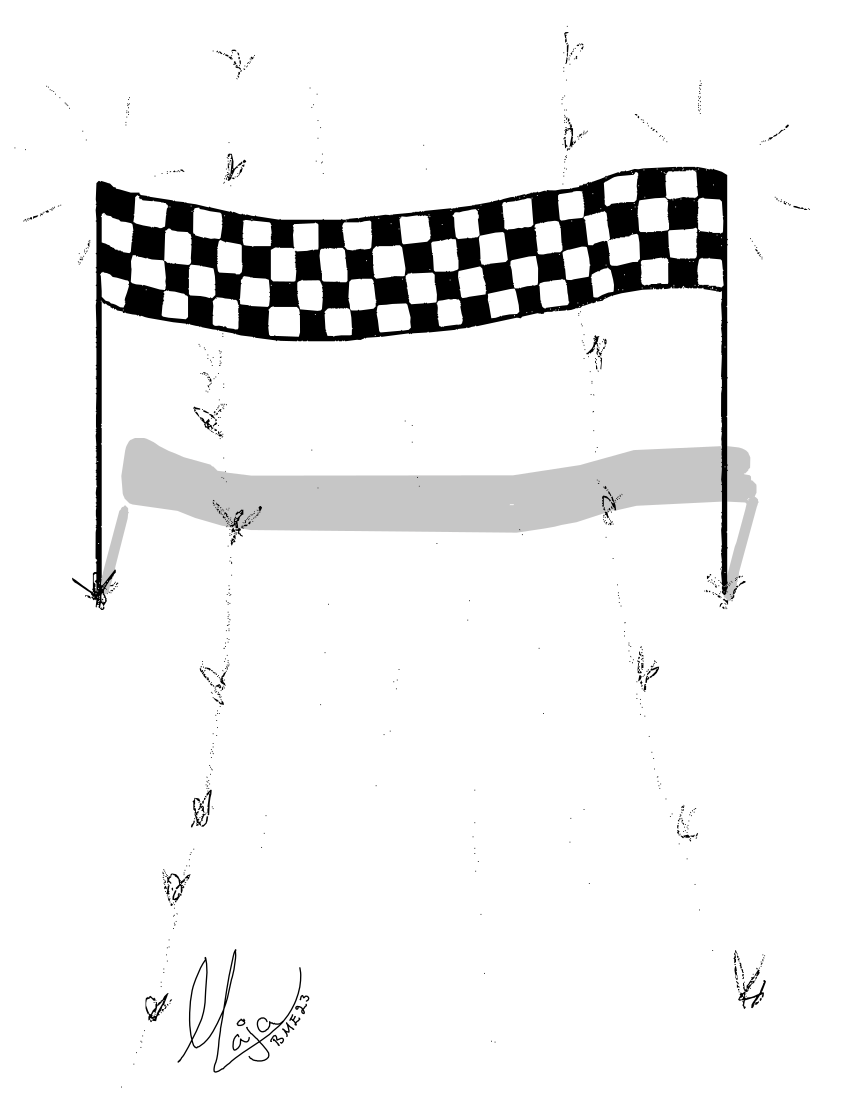
\includegraphics[width=1.5cm]{./bilder/majas-bilder/malgang.png}
\end{textblock*}



\begin{parse lines}[\noindent]{#1\\}
    Late one night, an engineer was lost in work and toil,
    He set off to find a darling girl to help discharge his coil
    In no time at all he'd warmed her up, her resistance at a low...
    They fluxed until the morning's light, when their fuses, they did blow

    We saved our dough for years to send the kid to MIT
    Although we knew it was a place of wild depravity
    But now we know our kid is safe and we should have no fear
    He's never even heard of Sex 'cause he's an engineer

    An MIT computer man got drunk one fateful night
    He opened up the console and smashed everything in sight
    When they finally subdued him, the judge he stood before,
    Said, "Lock him up for twenty years, he's rotten to the core!"

    Godiva was a lady well-endowed, there was no doubt
    She never wore a stitch of clothes, just wound her hair about
    The first man who did make her was an Engineer of course,
    But on just one drink, an Artsie queer had made Godiva's horse
    
    A maiden and an Engineer were sitting in the park
    The Engineer was working on some research after dark
    His scientific method was a marvel to observe
    While his right hand wrote the figures, his left hand traced the curves
\end{parse lines}

\vissteduatt{Visste du att The Engineers' Drinking Song är en väldigt lång sång?}

\newpage

